\subsection{Diagramy sekwencji}
\begin{adjustwidth}{2em}{0pt}

W tym podrozdziale przedstawiono wybrane diagramy sekwencji. Diagram sekwencji obrazuje interakcje pomiędzy częściami systemu w postaci sekwencji komunikatów np. wywołań funkcji wymienianych między nimi. 

\begin{figure}[H]
    \centering
    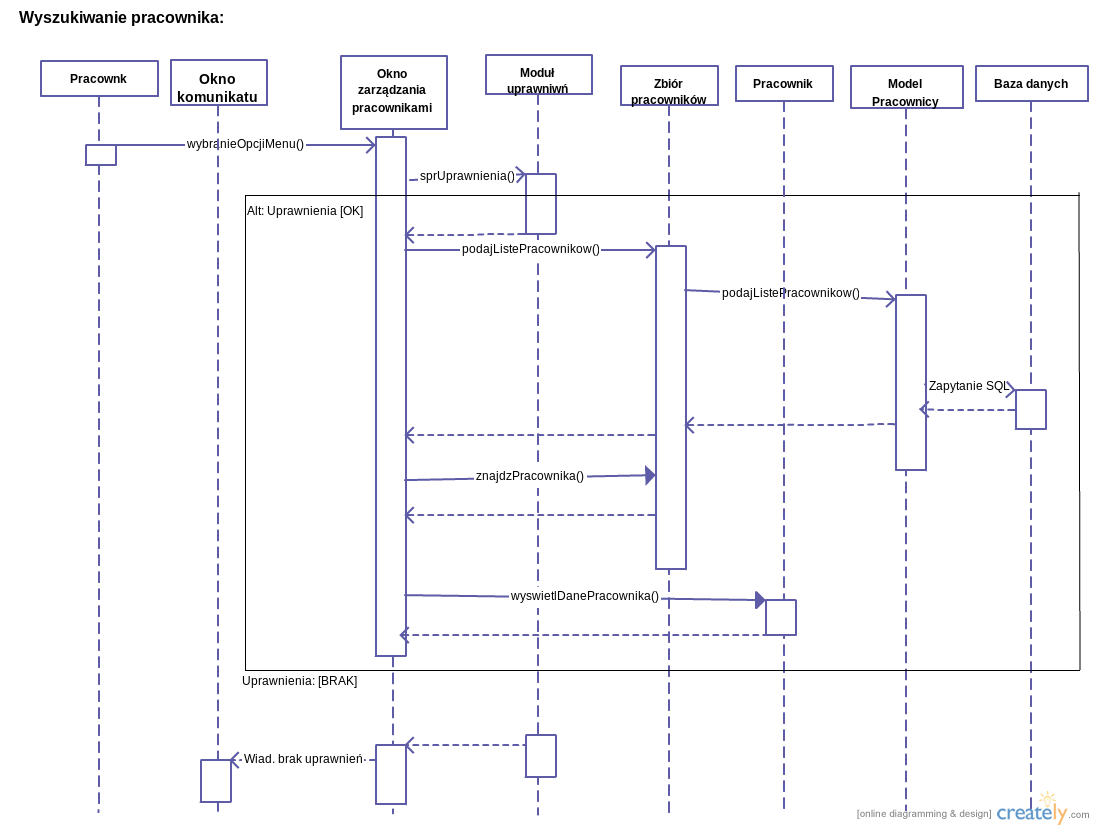
\includegraphics[scale=0.5, , angle=90 ]{./diagramy/sekwencji_i_komponentow/wyszukiwanie_pracownika.png}
    \caption{Diagram sekwencji: Wyszukiwanie pracownika}
    \label{fig:wyszukiwanie_pracownika}
\end{figure} 

\begin{figure}[H]
    \centering
    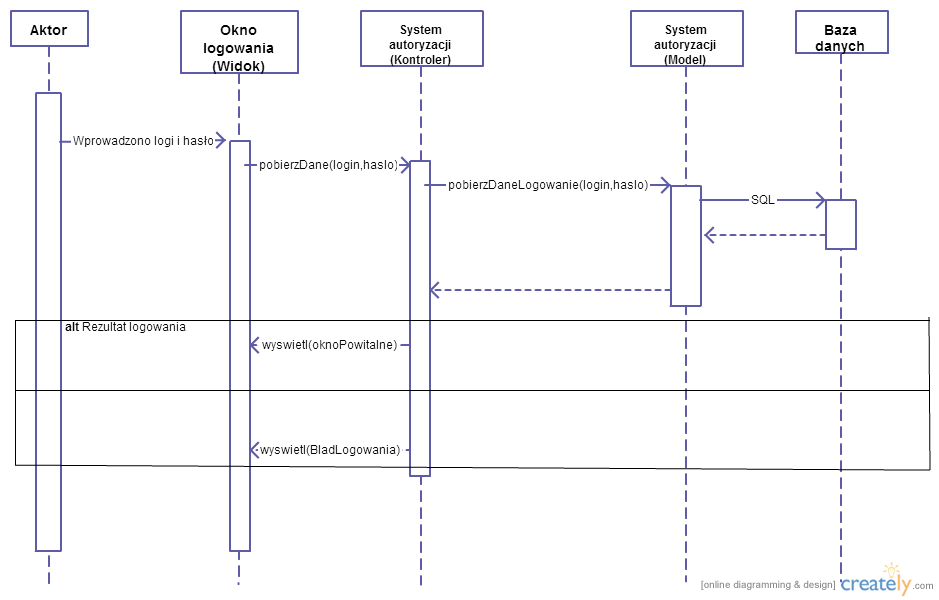
\includegraphics[scale=0.5]{./diagramy/sekwencji_i_komponentow/diag_sekwencji_logowanie.png}
    \caption{Diagram sekwencji: Logowanie do systemu}
    \label{fig:diag_sekwencji_logowanie.png}
\end{figure} 

\end{adjustwidth}
